\section{Elasticity reduction factor}\label{sec:exp-reduction-factor}

We introduced Hertz theory in \S~\ref{hertzTheory}, and now we apply it to experiments for analysis of ceramic pebbles. The derivation of Hertz force can be found on page~\pageref{eq:hertzForce} but is given again here for reference.
\begin{align*}
F = \frac{4}{3}E^*\sqrt{R^*}\,\delta^{3/2}
\end{align*}
and, again, the relative Young's modulus and radius are
\begin{align*}
\frac{1}{E^*} & = \frac{1-\nu_i^2}{E_i} + \frac{1-\nu_j^2}{E_j} \\
\frac{1}{R^*} & = \frac{1}{R_i} + \frac{1}{R_j}
\end{align*}

In experiments where we press a ceramic pebble between two platens, we measure the travel, $s$, rather than the pebble overlap, so we modify Eq.~\ref{eq:hertzForce} to be represented in terms of travel ($s = 2\delta$). Furthermore, for a pebble ($R_i = R_p$) in contact with a smooth plane ($R_j \rightarrow \infty$), the relative radius is simply $R^* = R_p = d_p/2$.

The Hertz force is now expressed as
\begin{align}\label{eq:contact-force}
F& = \frac{1}{3}E^*\sqrt{d_ps^3}
\end{align}

Let's take a moment to discuss Eq.~\ref{eq:contact-force}. The Young's modulus of the test stand platen is a constant value. One might assume the Young's modulus of the ceramic is also a known, constant value. In that case, there should be only a single force response for every pebble of a given diameter. Using the material properties given in Ref.~\cite{Gierszewski1998} for \lit, we plot a set of parametric curves based on diameter. The properties used for an nickel-alloy platen and \lit are given in Table~\ref{tab:hertz-dp-study-props}. The curves are given in Fig.~\ref{fig:hertz-dp-dependence}.

\begin {table}[htp] %
\caption{Material properties used for \lit and nickel-alloy platen}
\label {tab:hertz-dp-study-props} \centering %
\begin {tabular}{ cccccc }
\toprule %
$E_\text{peb}$		&     $\nu_\text{peb}$	&	$E_\text{stand}$		&     $\nu_\text{stand}$	\\
(GPa)			&					&	(GPa)				&					\\\toprule
126				&	0.24				&	220					& 	0.27				\\\bottomrule
\end{tabular}
\end{table}

\begin{figure}[ht!]
\centering
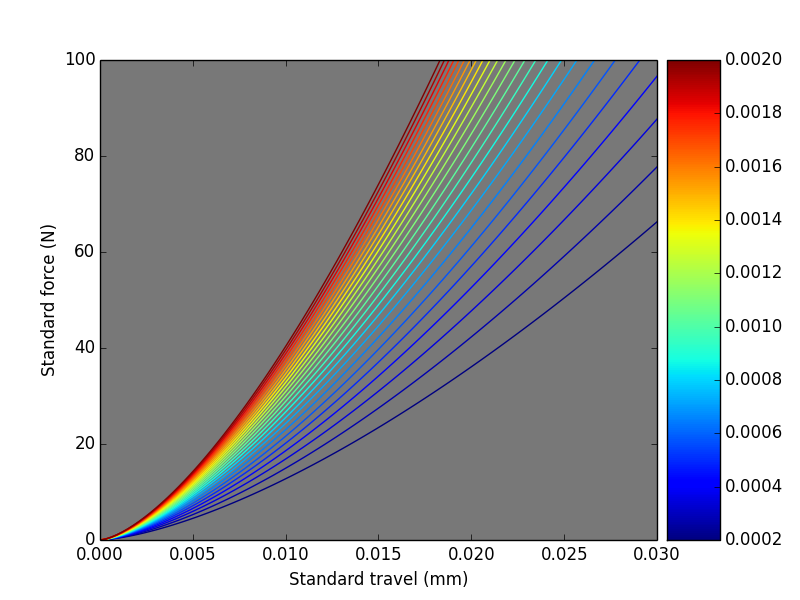
\includegraphics[width = 0.75 \textwidth]{chapters/figures/hertz-dp-dependence}
\caption{Hertzian responses of \lit pebbles compressed between platens. The colormap shows pebble diameters in \si{m}. The diameters span an order of magnitude from $d_p = \si{0.2 mm}$ to $d_p = \si{2 mm}$.}\label{fig:hertz-dp-dependence}
\end{figure}

Figure~\ref{fig:hertz-dp-dependence} clearly shows that if a pebble of a given diameter is strictly obeying Hertz theory, there is only a single force-displacement curve it can follow. However, when experiments are performed on single pebbles we see quite different behavior for the F-s curves, see the curves of Fig.~\ref{fig:exp-curves}. 

\begin{figure}
        \centering
        \begin{subfigure}[b]{0.75\textwidth}
                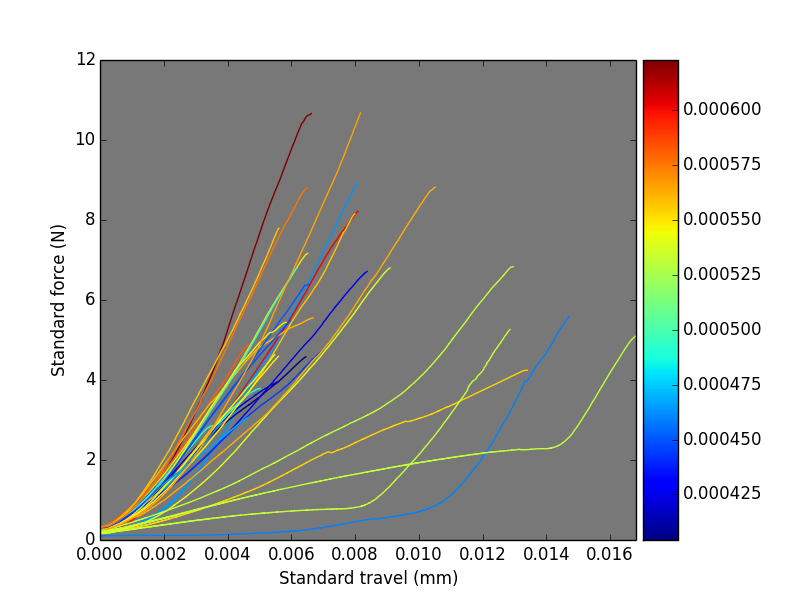
\includegraphics[width=\textwidth]{chapters/figures/fzk-exp-colormap}
                \caption{\lis pebbles of approximately \si{0.5 mm} diameter.}
                \label{fig:fzk-exp-colormap}
        \end{subfigure}
         
        %add desired spacing between images, e. g. ~, \quad, \qquad, \hfill etc.
        %(or a blank line to force the subfigure onto a new line)
        \begin{subfigure}[b]{0.75\textwidth}
                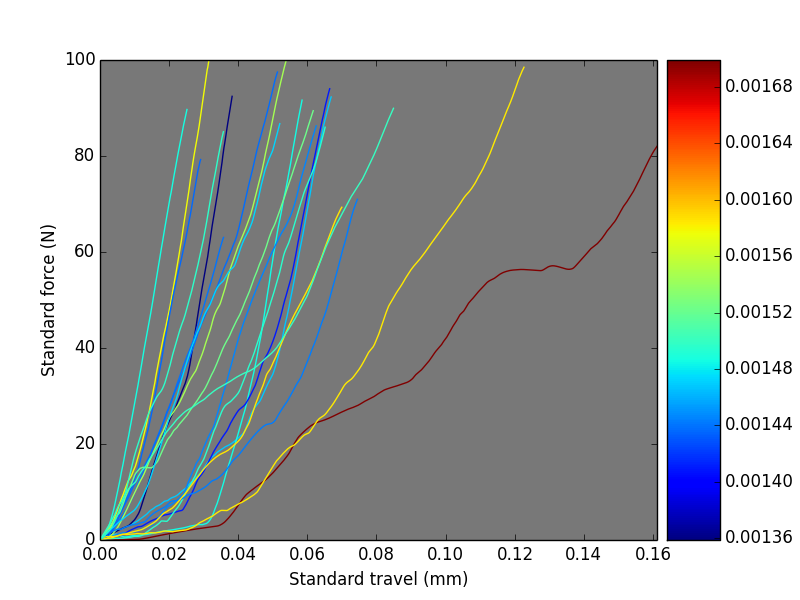
\includegraphics[width=\textwidth]{chapters/figures/nfri-exp-colormap}
                \caption{\lit pebbles of approximately \si{1.5 mm} diameter.}
                \label{fig:nfri-exp-colormap}
        \end{subfigure}
        \caption{Force-displacement curves for two sets of experimental data, a batch of \lis pebbles and a batch of \lit pebbles. The colormap shows pebble diameters in \si{m}.}\label{fig:exp-curves}
\end{figure}

Figure~\ref{fig:fzk-exp-colormap} shows \lis pebbles as they are compressed between platens. Neglecting the handful of pebbles with very low force responses to high strain, there is a grouping of pebbles where there is a general trend that matches Fig.~\ref{fig:hertz-dp-dependence}. The smaller diameter pebbles, in blue colors, have lower force responses for a given strain. Larger pebble diameters, in yellow-orange, are slightly higher overall in their force response. Finally, the largest diameter pebble in dark red has the highest force response for a given diameter. However, while the trends are \textit{generally} similar to the theoretical Hertzian curves, there are noticeable spreads in responses. The responses of \lit pebbles of Fig.~\ref{fig:nfri-exp-colormap}, on the contrary, show almost no adherence to the expected diameter dependence of Hertz theory. 

The behavior of pebbles observed in Fig.~\ref{fig:exp-curves} lead us to conclude that variations in pebble diameter can not alone account for the variation in the F-s curves. The most reasonable source for is a variation is in the Young's modulus of pebbles in a batch. Such a conclusion is important for implementation of Hertz theory in DEM algorithms.

We hypothesize that variation in the apparent Young's modulus of each pebble is rooted in the production of the pebbles which yields pebbles with slightly different internal structures. The differences in internal structure then cause the pebble to behave with different stiffnesses than the value expected from measurements of sintered pellets of lithium ceramics. In fact, we consider the sintered pellet Young's modulus, $E_\text{sp}$, as the upper limit for the pebbles and that most will emerge with values less than $E_\text{sp}$. To quantify the deviation of each pebble's $E_\text{peb}$ from the sintered pellet, we introduce a $k$ factor, defined as the elasticity reduction factor:
\begin{align}
k = \frac{E_\text{peb}}{E_\text{sp}}
\end{align}
where
\[
k \in [0,1]
\]

If each pebble has a unique $k$ value, this would quantify the spread in elastic responses seen in the experiments. We find the value by assuming that the pebbles are, in fact, behaving in a Hertzian manner. This allows us to back-out a $k$ value, or in other words the unique $E_\text{peb}$ of that pebble by finding a best fit to the experimental curves. 

We take the sintered pebble value of Young's modulus for \lis to be $E_\text{sp} = \si{90 GPa}$ and the value for \lit to be $E_\text{sp}= \si{124 GPa}$. Then we iterate over all values of $k\in[0,1]$ and compare the Hertzian response to that pebbles force-displacement curve. At each iteration, the L2-norm of the difference between Hertzian and experimental curves is used as the `error'. The L2 norm, $A$ for a given array, $a$ is 
\begin{align}
||A||_F = \left[\sum_{i,j}\textrm{abs}(a_{i,j})^2\right]^{1/2}
\end{align}

This is a convenient way to compare the error at every point along the force-displacement curves. When the error is minimized, the elasticity reduction value corresponding the minimum is recorded for that pebble. The Hertzian curves (in black) for each pebble are plotted in green against the experimental curves in Fig.~\ref{fig:exp-hertz}. 




\begin{figure}
        \centering
        \begin{subfigure}[b]{0.75\textwidth}
                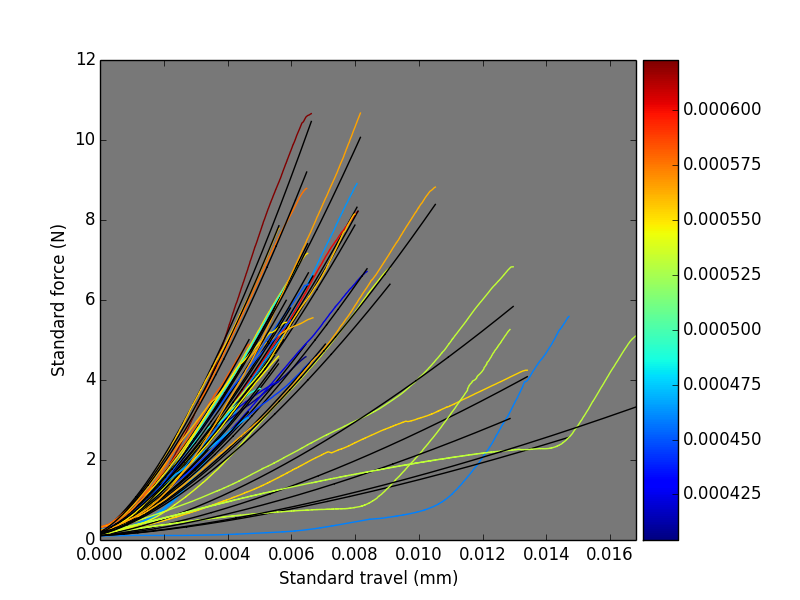
\includegraphics[width=\textwidth]{chapters/figures/fzk-hertz-colormap}
                \caption{\lis pebbles of approximately \si{0.5 mm} diameter.}
                \label{fig:fzk-hertz-colormap}
        \end{subfigure}
         
        %add desired spacing between images, e. g. ~, \quad, \qquad, \hfill etc.
        %(or a blank line to force the subfigure onto a new line)
        \begin{subfigure}[b]{0.75\textwidth}
                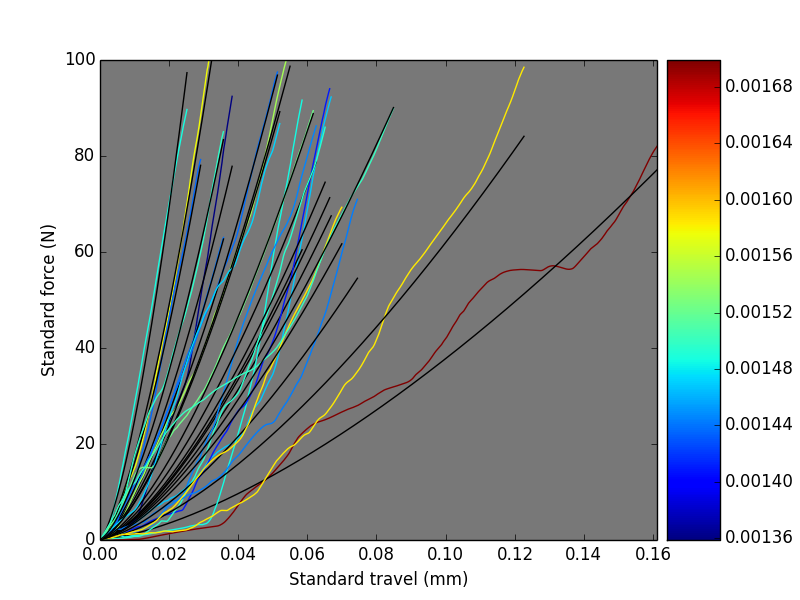
\includegraphics[width=\textwidth]{chapters/figures/nfri-hertz-colormap}
                \caption{\lit pebbles of approximately \si{1.5 mm} diameter.}
                \label{fig:nfri-hertz-colormap}
        \end{subfigure}
        \caption{Force-displacement curves for two sets of experimental data, a batch of \lis pebbles and a batch of \lit pebbles. The colormap shows pebble diameters in \si{m}.}\label{fig:exp-hertz}
\end{figure}



Many of the curves in Fig.~\ref{fig:fzk-hertz-colormap} seem to be fit well with a Hertzian curve with modified Young's modulus. The value of Young's modulus found for each pebble is plotted in Fig.~\ref{fig:fzk-E-plot}. The Young's modulus of pebble numbers 0 to 4 are the very 'soft' pebbles seen with very low forces on Fig.~\ref{fig:fzk-hertz-colormap}. The majority of pebbles behave with a Young's modulus between 30 and 70 \si{GPa}. On the upper end, a few pebbles acted very similar to their sintered pellet counterpart with approximate value of \si{90 GPa}.

\begin{figure}[ht!]
\centering
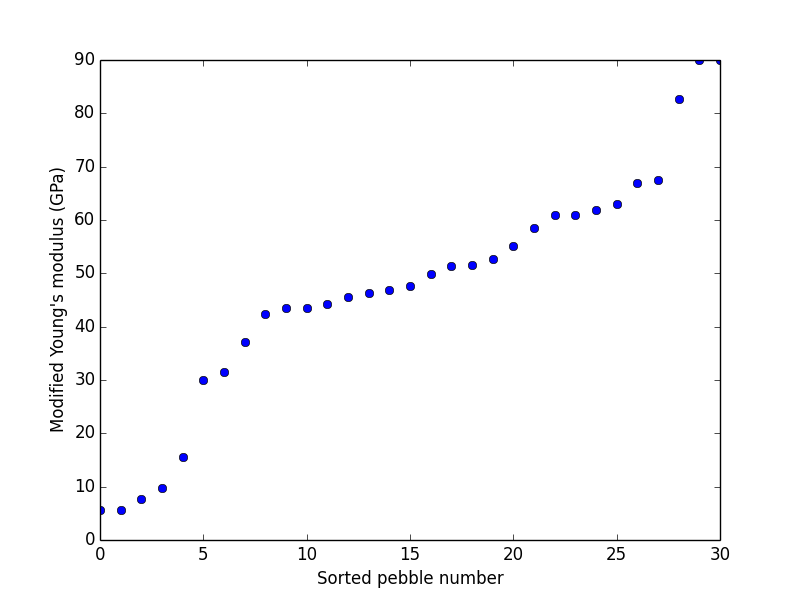
\includegraphics[width = 0.75 \textwidth]{chapters/figures/fzk-E-plot}
\caption{Distribution of modified Young's modulus for a batch of \lis pebbles. Most pebbles responded to compression with a Young's modulus well below the sintered pellet value of \si{90 GPa}.}\label{fig:fzk-E-plot}
\end{figure}

\begin{figure}[ht!]
\centering
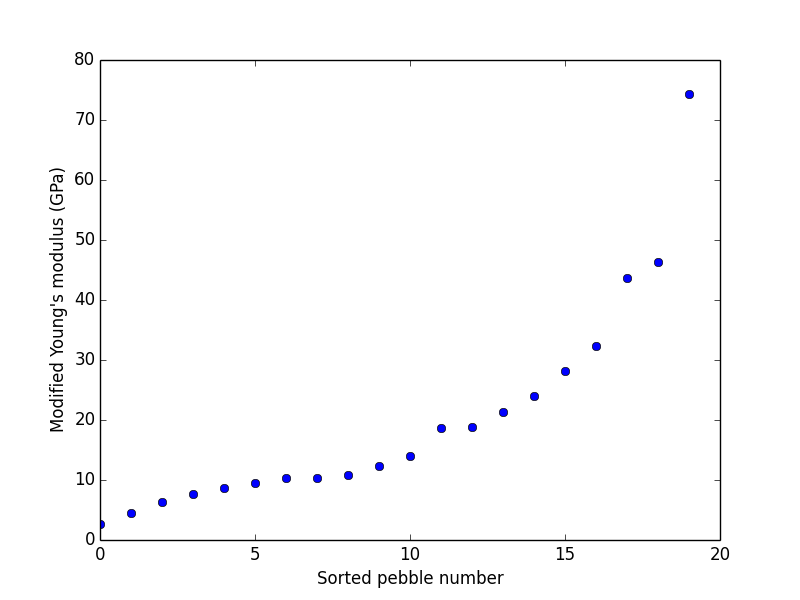
\includegraphics[width = 0.75 \textwidth]{chapters/figures/nfri-E-plot}
\caption{Distribution of modified Young's modulus for a batch of \lit pebbles. All pebbles responded to compression with a Young's modulus well below the sintered pellet value of \si{126 GPa}.}\label{fig:nfri-E-plot}
\end{figure}


What remains is actually using these modified Young's modulus in DEM simulations to see if they more accurately reflect pebble bed macroscopic behavior. If so, it is assumed they will more accurately reflect the contact forces between pebbles in the ensemble.



